\documentclass[letterpaper,12pt]{article}
\usepackage[T1]{fontenc}
\usepackage[utf8]{inputenc}
\usepackage{amsmath, amsfonts}
\usepackage{siunitx}
\usepackage{chemformula}

% remove spacing around date and author
\usepackage{titling}
\predate{}
\postdate{}
\preauthor{}
\postauthor{}

\author{}
\title{MATH 341 - Homework 1.2}
\date{} % clear date

\begin{document}

\maketitle

\begin{enumerate}
  \item[11.]
    The accompanying specific gravity values for various wood types used in construction appeared in the article ``Bolted Connection Design Values Based on European Yield Model'' (\textit{J. of Structural Engr., 1993: 2169-2186}):
    \begin{center}
      \begin{tabular}{l l l l l l l l l}
        .31 & .35 & .36 & .36 & .37 & .38 & .40 & .40 & .40 \\
        .41 & .41 & .42 & .42 & .42 & .42 & .42 & .43 & .44 \\
        .45 & .46 & .46 & .47 & .48 & .48 & .48 & .51 & .54 \\
        .54 & .55 & .58 & .62 & .66 & .66 & .67 & .68 & .75
      \end{tabular}
    \end{center}
    Construct a stem-and-leaf display using repeated stems, and comment on any interesting features of the display.
    \begin{center}
      \begin{tabular}{c | c c c c c c c c c c c c c c c c c c c}
        % Stem & \multicolumn{19}{l}{Leaf} \\
        % \hline
        3 & 1 & 5 & 6 & 6 & 7 & 8 \\
        4 & 0 & 0 & 0 & 1 & 1 & 2 & 2 & 2 & 2 & 2 & 3 & 4 & 5 & 6 & 6 & 7 & 8 & 8 & 8 \\
        5 & 1 & 4 & 4 & 5 & 8 \\
        6 & 2 & 6 & 6 & 7 & 8\\
        7 & 5 \\
        \multicolumn{20}{r}{Key: 1 | 2 = 0.12}
      \end{tabular}
    \end{center}
    The display has one peak at stem 4. It suggests that a typical value is in stem 4, perhaps 0.42. The data is not quite symmetric since the larger values tend to be more stretched out than the smaller ones. There is a bit of a gap between the largest value and the rest of the data (0.68 versus 0.75).
  \item[12.]
    The accompanying summary data on \ch{CeO2} particle sizes (nm) under certain experimental conditions was read from a graph in the article ``Nanoceria – Energetics of Surfaces, Interfaces and Water Adsorption'' (\textit{J. of the Amer. Ceramic Soc.}, 2011: 3992–3999):
    \begin{center}
      \begin{tabular}{c c c c c}
        3.0-<3.5 & 3.5-<4.0 & 4.0-<4.5 & 4.5-<5.0 & 5.0-<5.5 \\
        5 & 15 & 27 & 34 & 22 \\
        5.5-<6.0 & 6.0-<6.5 & 6.5-<7.0 &  7.0-<7.5 & 7.5-<8.0 \\
        14 & 7 & 2 & 4 & 1
      \end{tabular}
    \end{center}
    \begin{enumerate}
      \item[a.]
        What proportion of the observations are less than 5?
      \item[b.]
        What proportion of the observations are at least 6?
      \item[c.]
        Construct a histogram with relative frequency on the vertical axis and comment on interesting features. In particular, does the distribution of particle sizes appear to be reasonably symmetric or somewhat skewed? [\textit{Note}: The investigators fit a lognormal distribution to the data; this is discussed in Chapter 4.]
      \item[d.]
        Construct a histogram with density on the vertical axis and compare to the histogram in (c).
    \end{enumerate}
  \item[17.]
    The accompanying data came from a study of collusion in bidding within the construction industry (``Detection of Collusive Behavior,'' \textit{J. of Construction Engr. and Mgmnt}, 2012: 1251–1258).
    \begin{center}
      \begin{tabular}{S[table-format=2.0]S[table-format=2.0]}
        \textbf{No. Bidders} & \textbf{No. Contracts} \\
        2 & 7 \\
        3 & 20 \\
        4 & 26 \\
        5 & 16 \\
        6 & 11 \\
        7 & 9 \\
        8 & 6 \\
        9 & 8 \\
        10 & 3 \\
        11 & 2
      \end{tabular}
    \end{center}
    \begin{enumerate}
      \item[a.]
        What proportion of the contracts involved at most five bidders? At least five bidders?
      \item[b.]
        What proportion of the contracts involved between five and 10 bidders, inclusive? Strictly between five and 10 bidders?
      \item[c.]
        Construct a histogram and comment on interesting features.
    \end{enumerate}
  \item[19.]
    The number of contaminating particles on a silicon wafer prior to a certain rinsing process was determined for each wafer in a sample of size 100, resulting in the following frequencies:
    \begin{center}
      \begin{tabular}{
        l
        S[table-format=2.0]
        S[table-format=2.0]
        S[table-format=2.0]
        S[table-format=2.0]
        S[table-format=2.0]
        S[table-format=2.0]
        S[table-format=2.0]
        S[table-format=2.0]
      }
        \textit{Number of particles} & 0 & 1 & 2 & 3 & 4 & 5 & 6 & 7 \\
        \textit{Frequency} & 1 & 2 & 3 & 12 & 11 & 15 & 18 & 10 \\
        \textit{Number of particles} & 8 & 9 & 10 & 11 & 12 & 13 & 1 \\
        \textit{Frequency} & 12 & 4 & 5 & 3 & 1 & 2 & 1
      \end{tabular}
    \end{center}
    \begin{enumerate}
      \item[a.]
        What proportion of the sampled wafers had at least one particle? At least five particles?
      \item[b.]
        What proportion of the sampled wafers had between five and ten particles, inclusive? Strictly between five and ten particles?
      \item[c.]
        Draw a histogram using relative frequency on the vertical axis. How would you describe the shape of the histogram?
    \end{enumerate}
  \item[22.]
    How does the speed of a runner vary over the course of a marathon (a distance of 42.195 km)? Consider determining both the time to run the first 5 km and the time to run between the 35-km and 40-km points, and then sub-
    tracting the former time from the latter time. A positive value of this difference corresponds to a runner slowing down toward the end of the race. The accompanying histogram is based on times of runners who participated in several different Japanese marathons (``Factors Affecting Runners’ Marathon Performance,'' \textit{Chance, Fall}, 1993: 24–30).

    What are some interesting features of this histogram? What is a typical difference value? Roughly what proportion of the runners ran the late distance more quickly than the early distance?

    \begin{center}
      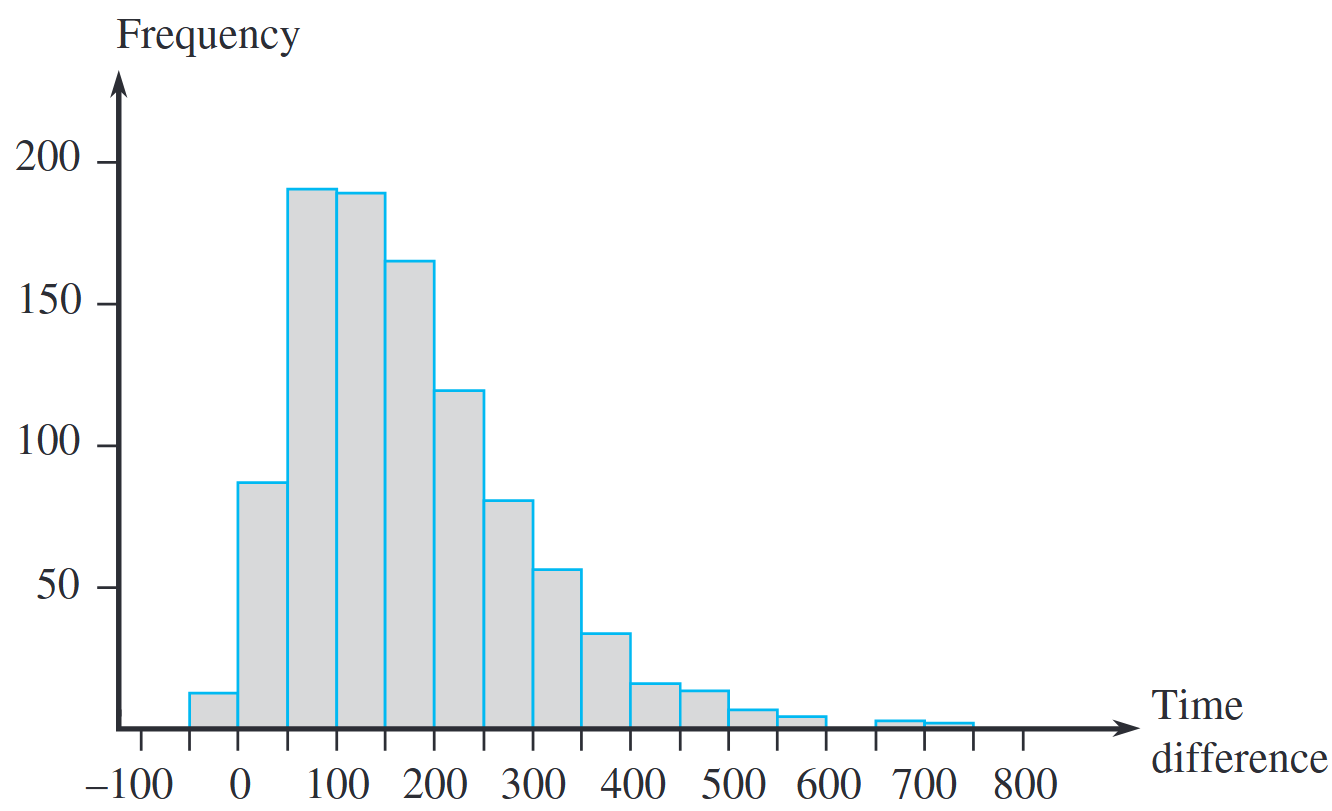
\includegraphics[scale=0.3]{../resources/01_02_22_01.png}
    \end{center}
\end{enumerate}

\end{document}
